\section{Introduction}

\begin{frame}{Introduction: Language Background}
\begin{itemize}
\item Nuuchahnulth (ISO 639-3 nuk, formerly Nootka) is a Wakashan language from the South Wakashan branch.
\item Native speakers are older, at least in part due to Canada's historic residential school policy.
\item Dialect continuum spoken among thirteen tribes along the west coast of Vancouver Island
\item Following \cite{werle2013dialects}, I break into four broad dialect groups.
\end{itemize}
\end{frame}

\begin{frame}

%\begin{figure}
%\centering
%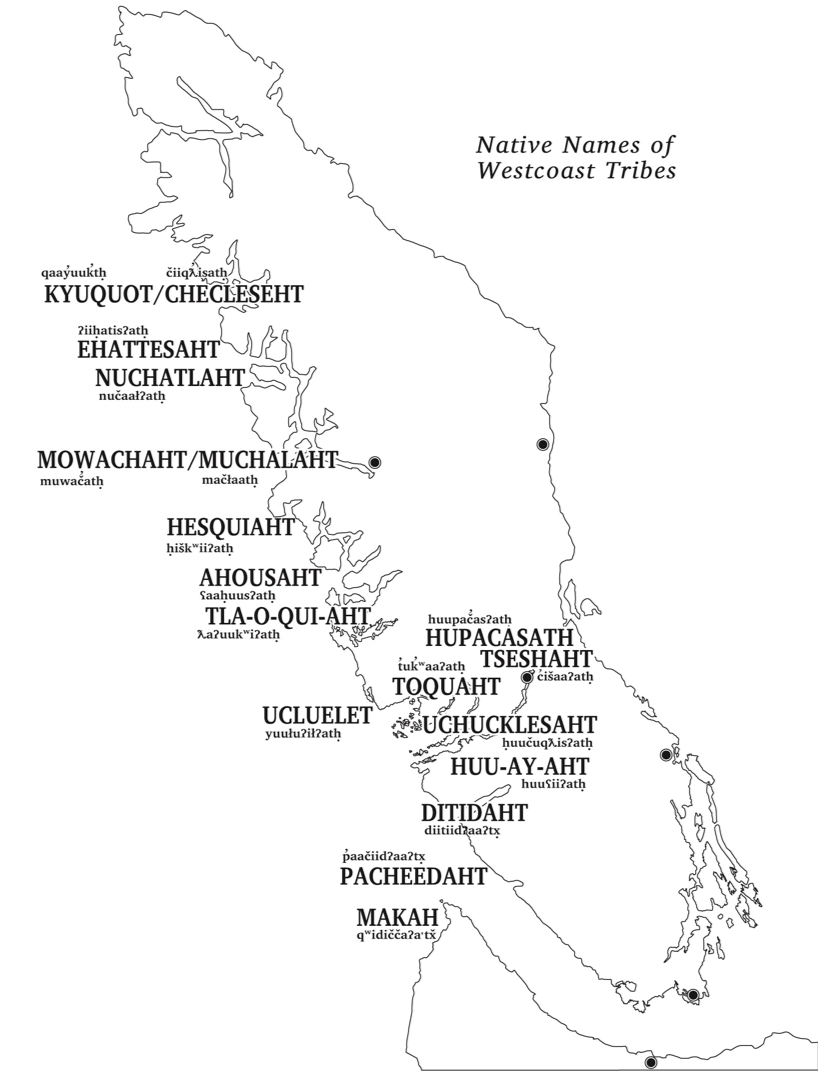
\includegraphics[height=\paperheight]{ncn-map.png}
%\end{figure}

\begin{tikzpicture}[remember picture, overlay]
  \node [anchor = north] at (current page.north)
     {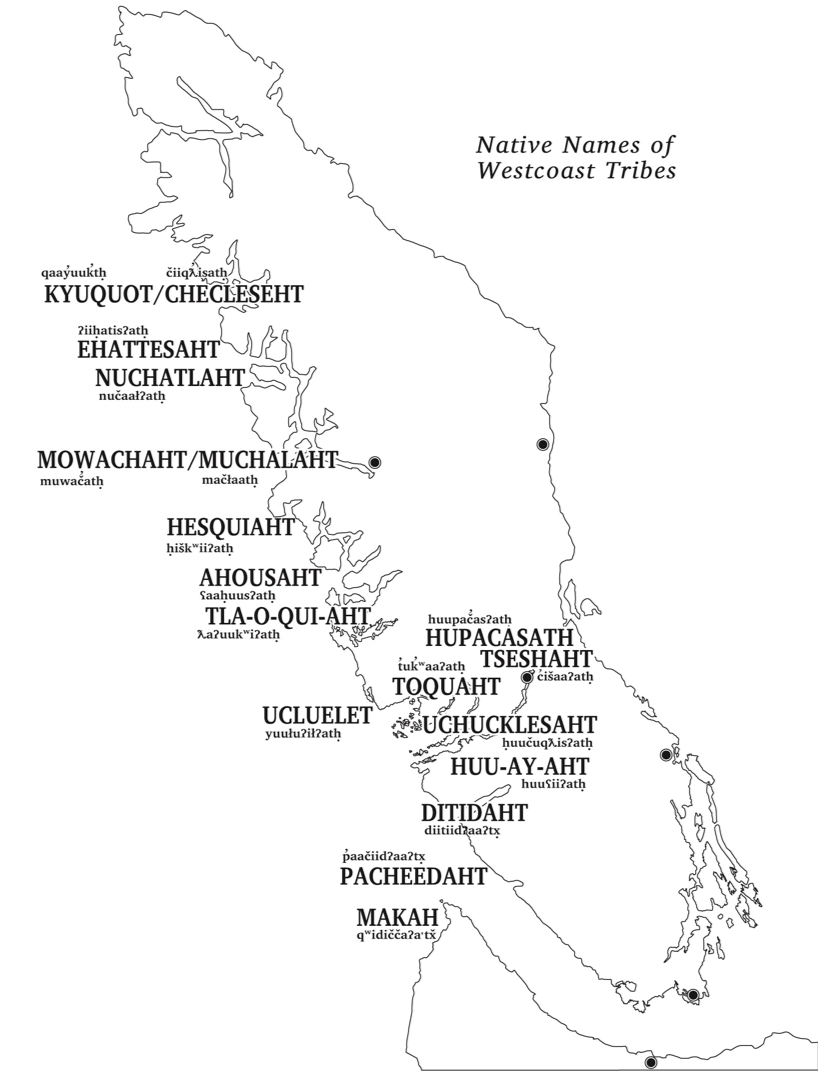
\includegraphics[height=\paperheight]{ncn-map.png}};
  \node [anchor=south west, inner sep=0pt]  at (current page.south west)
     {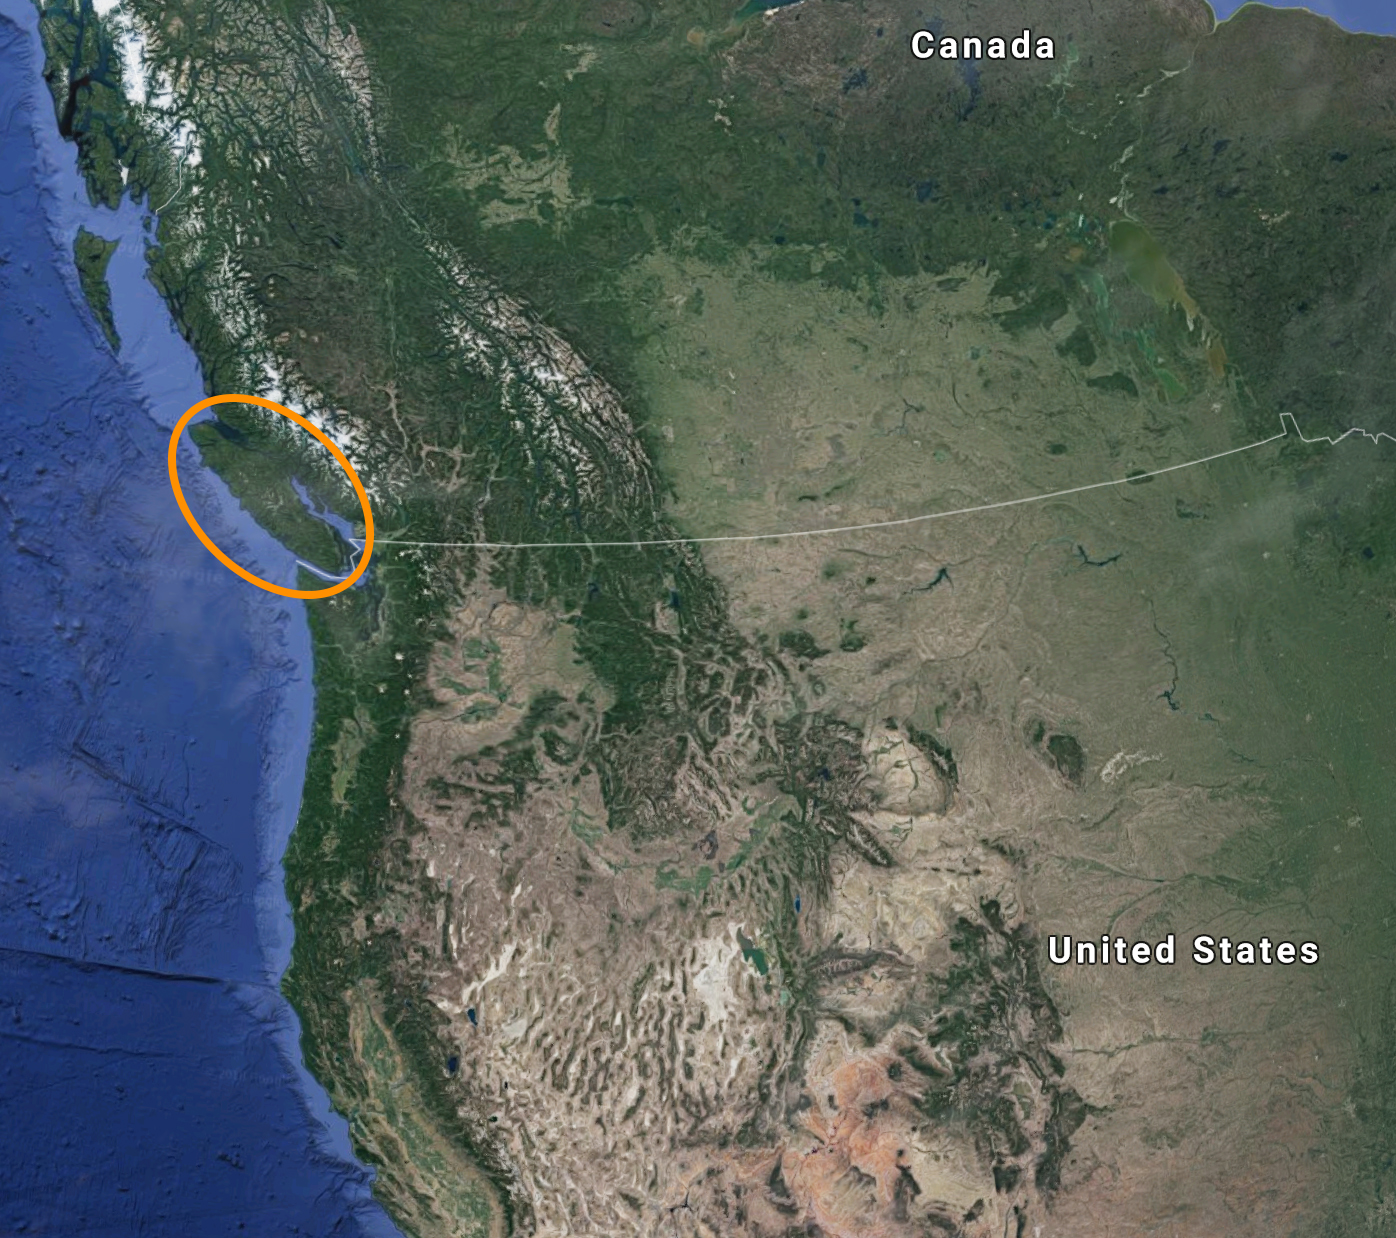
\includegraphics[height=3cm]{vanislandcircle.jpg}};
\end{tikzpicture}

\end{frame}

\begin{frame}

\begin{tikzpicture}[remember picture, overlay]
  \node [anchor = north] at (current page.north)
     {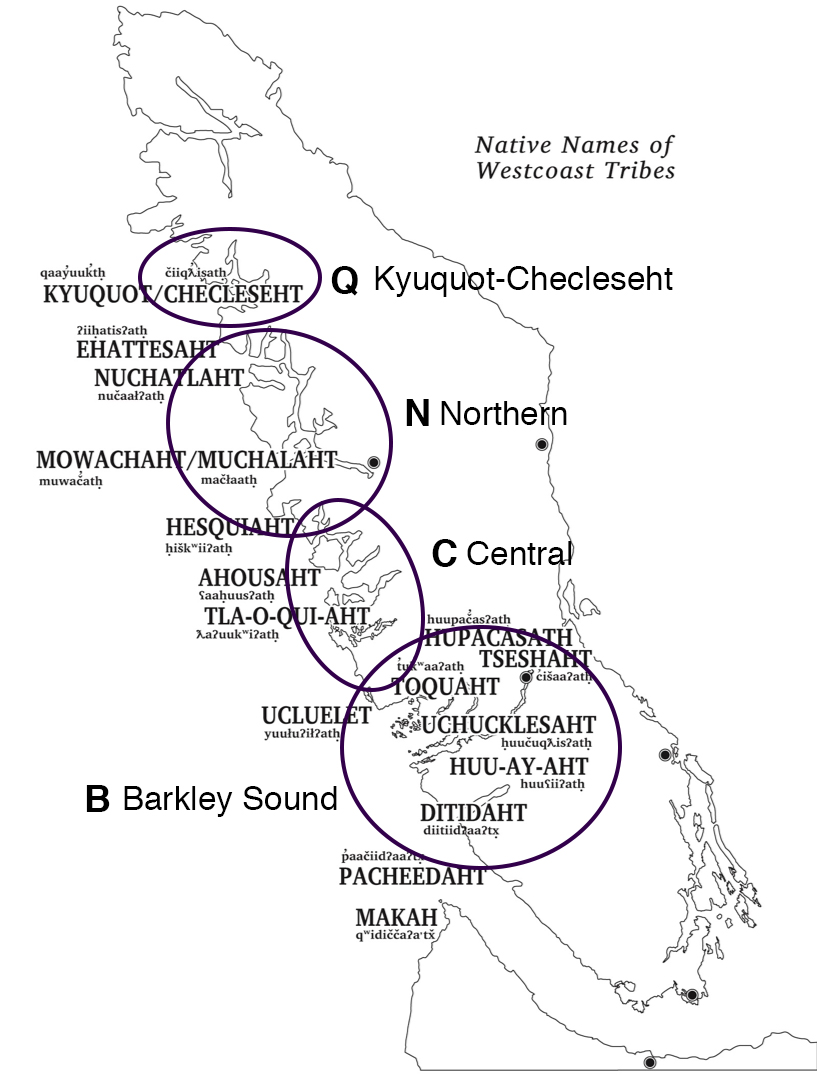
\includegraphics[height=\paperheight]{ncn-dialects.jpg}};
  \node [anchor=south west, inner sep=0pt]  at (current page.south west)
     {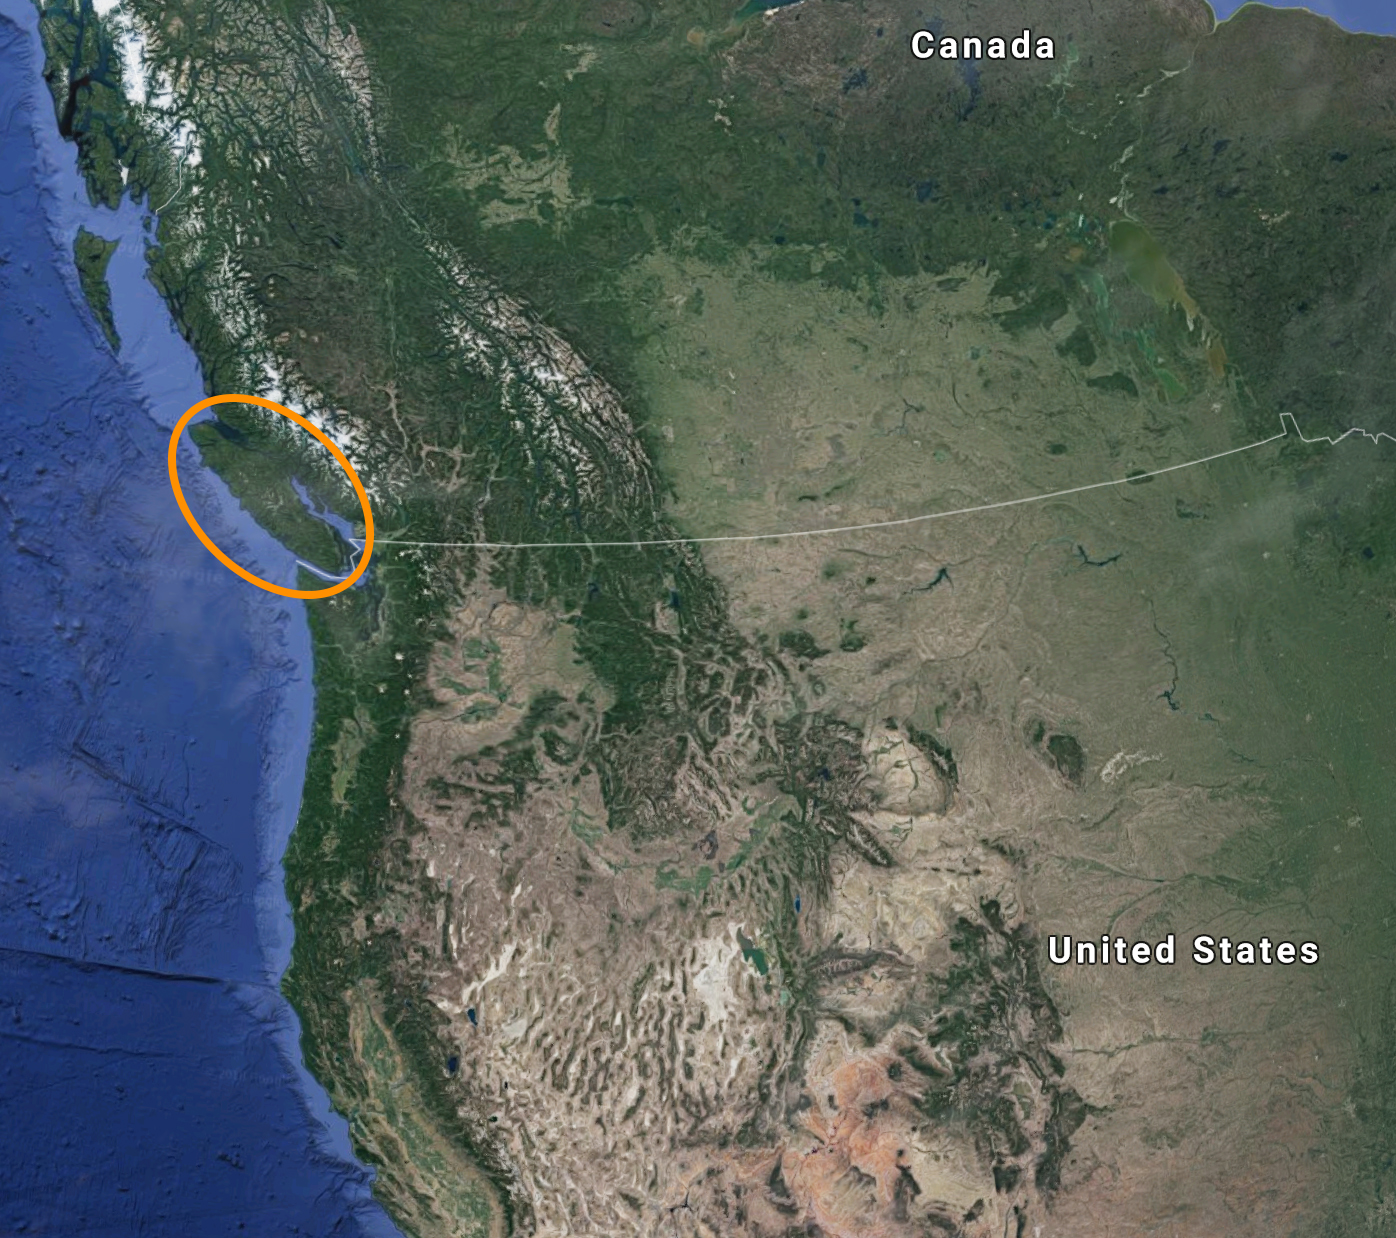
\includegraphics[height=3cm]{vanislandcircle.jpg}};
\end{tikzpicture}
\end{frame}

\begin{frame}{Introduction: Linguistic Background}
\begin{itemize}
\item Linguistic work dates to \cite{sapir1911}
\item Largest published texts in the Barkley Sound dialect \citep{sapir1939, sapir1955}
\item Recent syntactic work focused on the suffix ordering:
\begin{itemize}
\item \cite{waldie2004}: Suffix verbs (HPSG + linearization)
\item \cite{wojdak2005}: Suffix verbs (Minimalism)
\item \cite{woo2007b}: Adposition-like suffixes and argument-marking
\end{itemize}
\item Little analysis of the boundaries of clauses, clause/verb adjoining or coordination
\end{itemize}
\end{frame}

\begin{frame}{Methodology}
\begin{itemize}
\item Field work with speakers: describing images, question-answering, English translation, rephrasing, forced choice, linguist-constructed examples
\item Corpus study: Nootka Texts, community-produced texts, texts from other linguists, texts I collected from consultants
\item Analysis was done in an implemented DELPH-IN grammar, built using the HPSG formalism
\end{itemize}
\end{frame}